\label{Chapter Methodology} 
\section{Methodology}
    In this project, the YOLOv5 algorithm will be used to search for instances of specified objects in a given image.
    The general workflow is shown in the following figure.\\
    \begin{center}
    \captionsetup[figure]{name=Diagram}          
    \smartdiagram[circular diagram:clockwise]{Data Gathering, Data Preparation, Evolving Hyperparameters, Training, Inference, Manually Check Label}
    \captionof{figure}{Workflow}
\end{center}        
% ================================================================================================= 
        \subsection{Data Gathering}
            Image Variety, such as various lighting, perspectives, styles, and other factors was especially concentrated on to get the best forecast. 
            Hence, data are gathered across multiple sources from different artists.
            \subsubsection{Web-scraping}
    The main source for the images used for our dataset is \textbf{Pixiv} since it is one of the biggest communities for artists to draw and share artworks related to anime in particular.
    Takahiro Kamitani and Takanori Katagiri originally released it on September 10, 2007, as a beta test. 
    The headquarters of Pixiv Inc. are located in Sendagaya, Shibuya, Tokyo, Japan. 
    The website had more than 50 million users as of April 2020, received more than 100 million entries, and had more than 3.7 billion monthly page views. 
    The foundation of the website is an extensive tag structure that organizes the artwork.
    To make downloading a large number of images from Pixiv easier, a script based on \textbf{Powerful Downloader}\cite{PixivBatchDownloader} and \textbf{PixivUtil2}\cite{PixivUtil2} was created.
    
    Due to the scarcity of artwork for some lesser-known idols on Pixiv, the Youtube API to was used to crawl thumbnails from their youtube channels.
    Since this is a big company, the management team has done a very good job of design artwork, compose music as well as planning the schedule. 
    
    Last but not least, Twitter is the sub-source for this project as there are some talented artists who only publish their works on this platform since the website has a huge amount of traffic.
    Jack Dorsey, Noah Glass, Biz Stone, and Evan Williams founded Twitter in March 2006, and it went live in July of the same year. 
    With more than 25 offices worldwide, Twitter, Inc. is a California corporation with its headquarters in San Francisco. 
    By 2012, the service was handling an average of 1.6 billion search queries daily, with more than 100 million users posting 340 million tweets each day\cite{Twitter}.
    
    Mainly, scripts are using popular libraries to crawl data such as BeautifulSoup or Selenium.
            \subsubsection{Video to frames}
    In order to diversify the dataset, a custom program was created to take frame by frame from a given video and save them as an image file. 
    Because each second of the video contains approximately 24 frames, having too many similar frames becomes an issue.
    This is solved by incorporating Pearson's correlation coefficient into the program, which detects and eliminates similar frames automatically.
    \begin{center}
        \textbf{Pearson Correlation Coefficient}\cite{freedman2007statistics}
        \begin{equation*}
            r = \frac{\sum (x_{i}-\overline{x})(y_{i}-\overline{y})}{\sqrt{\sum (x_{i}-\overline{x})^2\sum (y_{i}-\overline{y})^2}}
        \end{equation*}
    \end{center}
        $r$	:	correlation coefficient\\
        $x_{i}$	:	values of the x-variable in a sample\\
        $\bar{x}$	:	mean of the values of the x-variable\\
        $y_{i}$	:	values of the y-variable in a sample\\
        $\bar{y}$	:	mean of the values of the y-variable\\
    Called the first frame the base image, calculate the correlation coefficient of the base image and the next frame. 
    If the score is larger than a given threshold, that next image will be deleted. And then the program will consider the next frame in the timeline until the video is over.
    
\begin{figure}[H]
    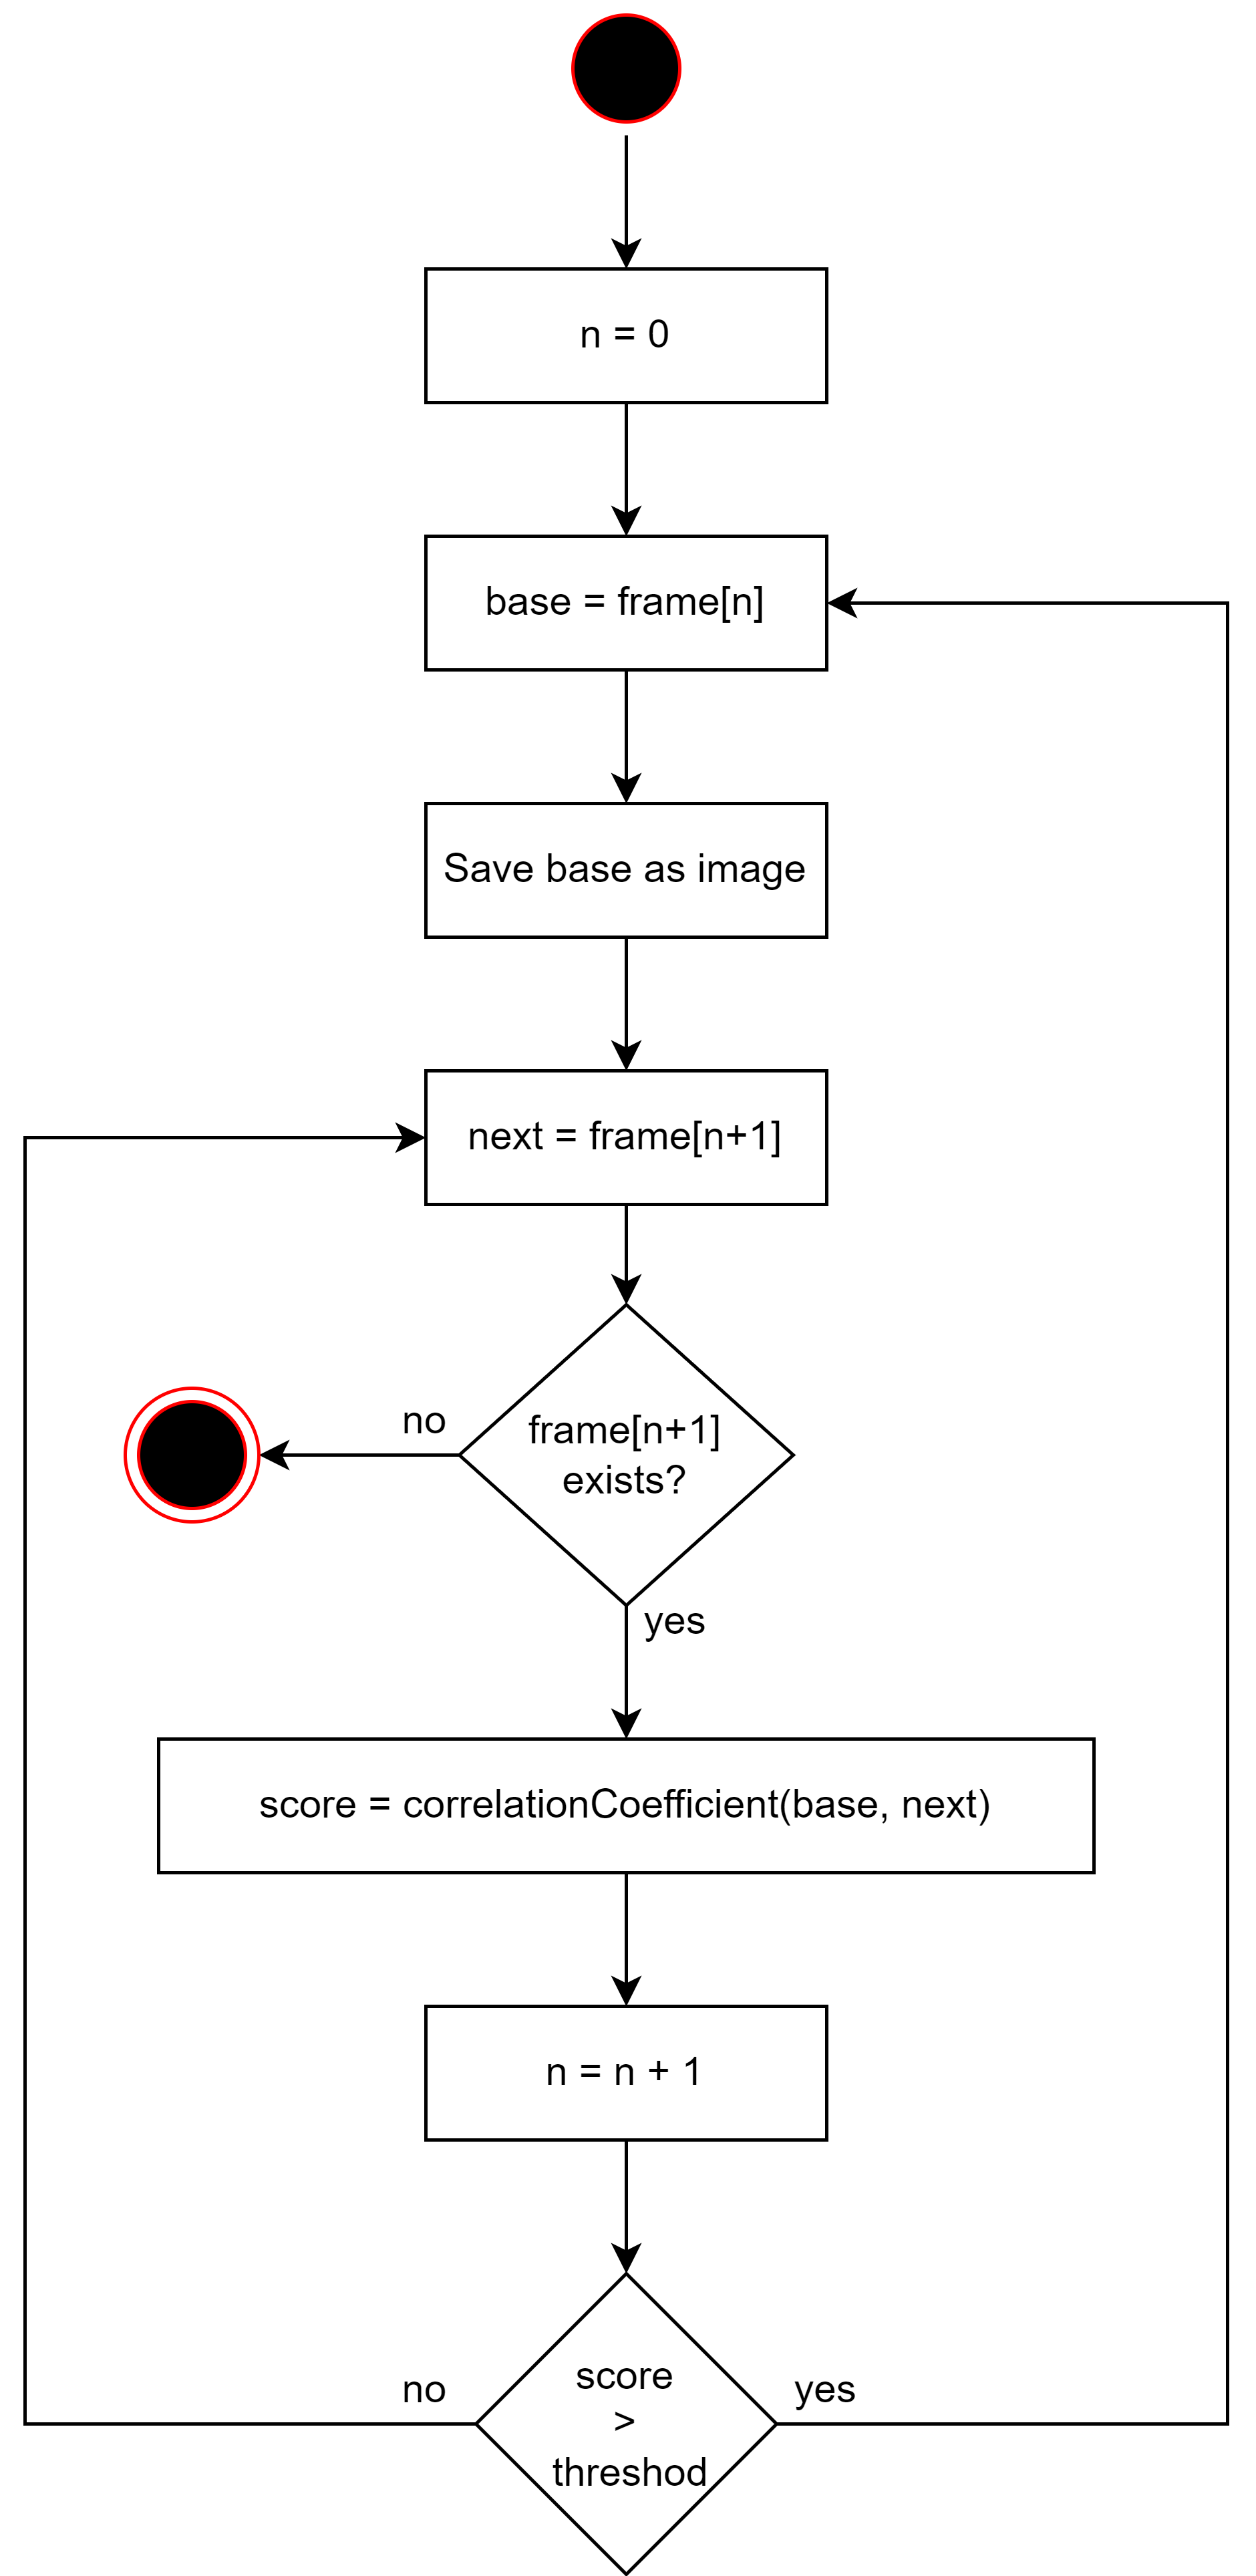
\includegraphics[width=0.5\textwidth]{diagrams/FlowChart-VideoToFrames.png}
    \caption{Video to frames flowchart}
    \end{figure}
% ================================================================================================= 
        \subsection{Data Preparation}
            During the collection of images to use for the dataset, certain classes had much more samples to choose from compared to others, which led to an imbalanced problem.
            Predictive modeling is challenged by imbalanced classifications since the majority of machine learning methods for classification were built on the premise that there should be an equal number of samples in each class. This is because most algorithms are intended to be as accurate and error-free as possible.
            However, if the data set is imbalanced, the model may still forecast the majority class with a high degree of accuracy but not the minority class, which is often the goal of the model in the first place.
            \subsubsection{Split Dataset}
    A customized under-sampling technique was used to avoid this situation. 
    The standard under-sampling technique does not meet the requirement simply due to the fact that many of the images used for the dataset have multiple labels.
    In other words, elimination of an image will lead to the perishment of many other labels.
    \paragraph{Calculating Quantity}
        Firstly, start with finding the lowest number of labels out of all the classes to set a standard upon which to divide a ratio between training, validating, and testing. The sum of the ratio of each dataset must be equal to 1:\\
        \begin{center}
            \(p(train) + p(val) + p(test) = 1\) 
        \end{center} 
        From that, calculate the number of labels per class needed in each subset by:
        \begin{center}
            \(n(train) = p(train) * standard\) \\
            \(n(val) = p(val) * standard\) \\
            \(n(test) = p(test) * standard\) 
        \end{center} 
    \paragraph{Customized Under-sampling Algorithm}
        The choose approach was employed as opposed to deleting. 
        The algorithm will first loop over all of the classes that are available. 
        After that, sort the dataset by how many labels there are in total for that class for each image. 
        The image will be chosen by an algorithm from left to right. 
        The image will be added to the new dataset if the total number of labels from each class does not exceed the predetermined number in the previous section (\autoref{fig:CustomizedUnderSampling}).
            \subsubsection{Data Augmentation}
    Generally, when using Machine Learning for classification problems, it is more ideal to learn a classifier that can perform well on a population. 
    An example of a population would be the set of all handwritten characters in the entire world. Generally, that complete population will not always be available for training, we only have a much smaller training dataset. 
    If a training set is large enough, it might be a good approximation of the population we're interested in, but it's still just that, an approximation.
    
    A learning algorithm is over-fitting if it performs significantly better on the training set than it is on the population (which will be generally approximated again using a separate test set).
    
    To help combat over-fitting and data deficiency, along with increasing the model's accuracy, Data Augmentation techniques are used to diversify existing data points.
    Data augmentation is an effective method for enhancing the performance of our computer vision models without having to collect more data.
    \label{Figure Data Augmentation}
\begin{figure}[H]
    \centering
    \begin{subfigure}{0.15\textwidth}
        \centering
        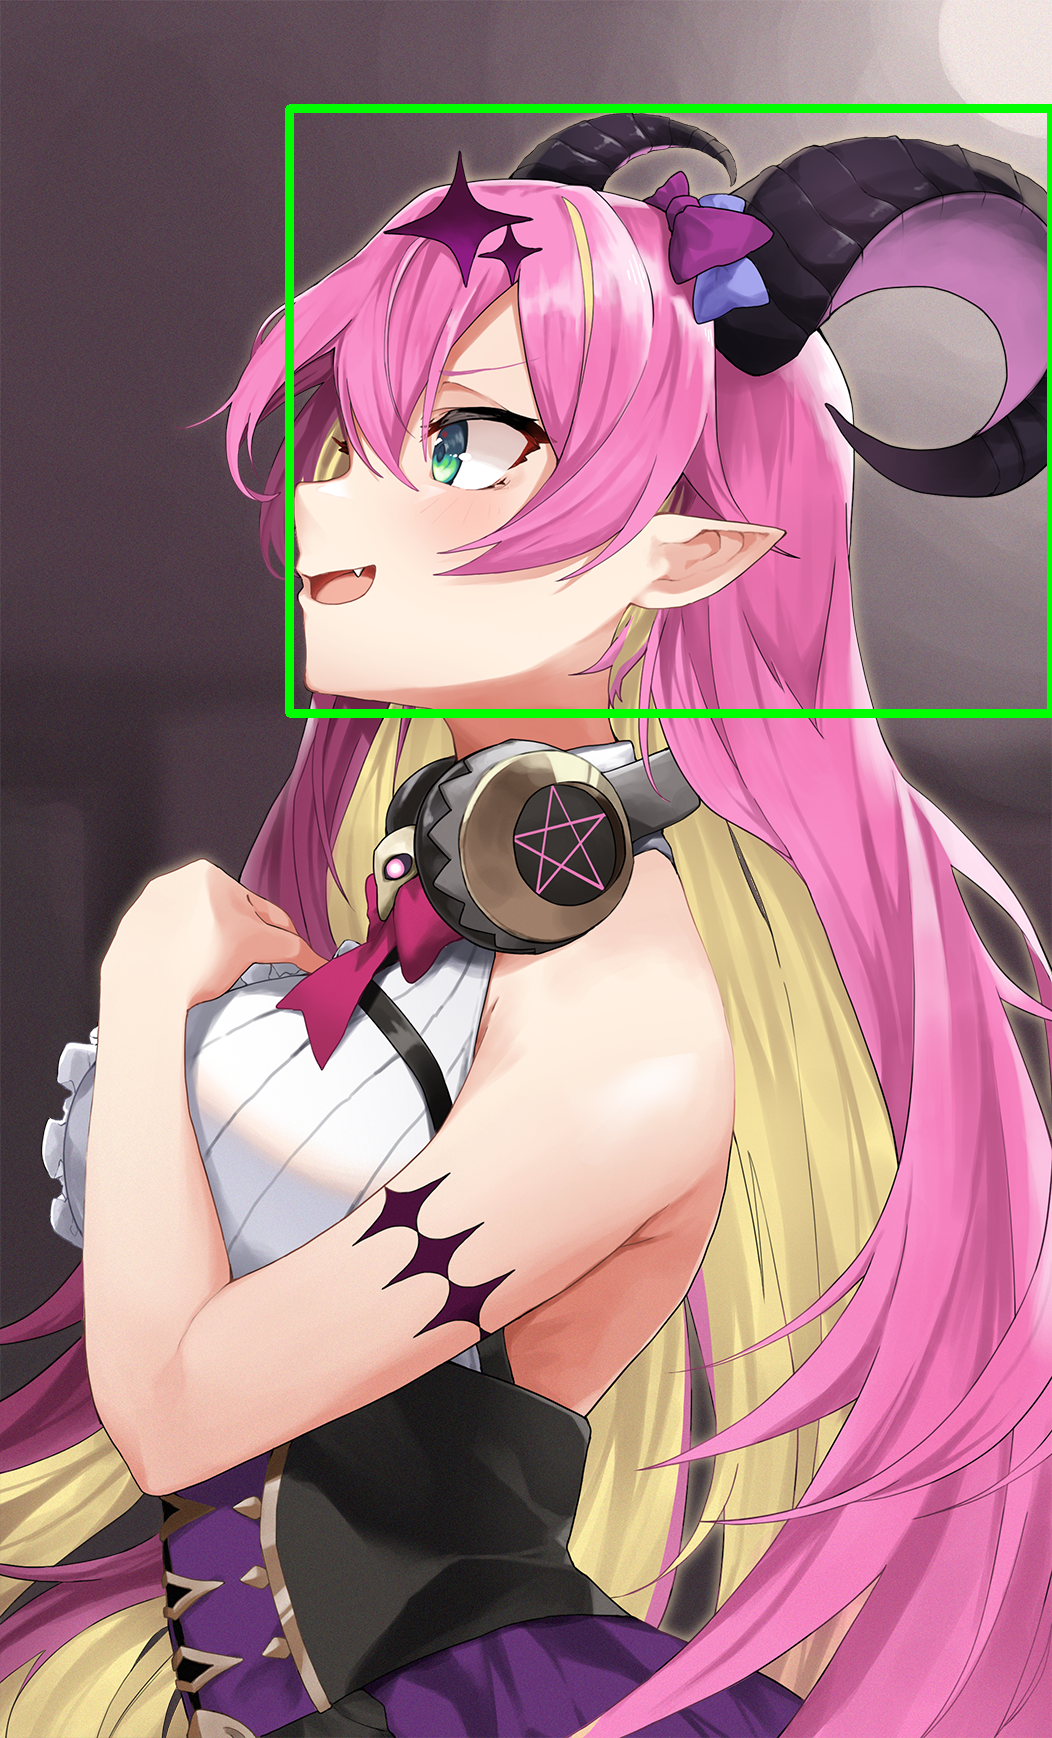
\includegraphics[width=\textwidth]{images/augmentation/Pixiv-83768702_p0-BB.png}
        \caption{}
        \label{fig:aloe1}
    \end{subfigure}
    \hfill
    \begin{subfigure}{0.15\textwidth}
        \centering
        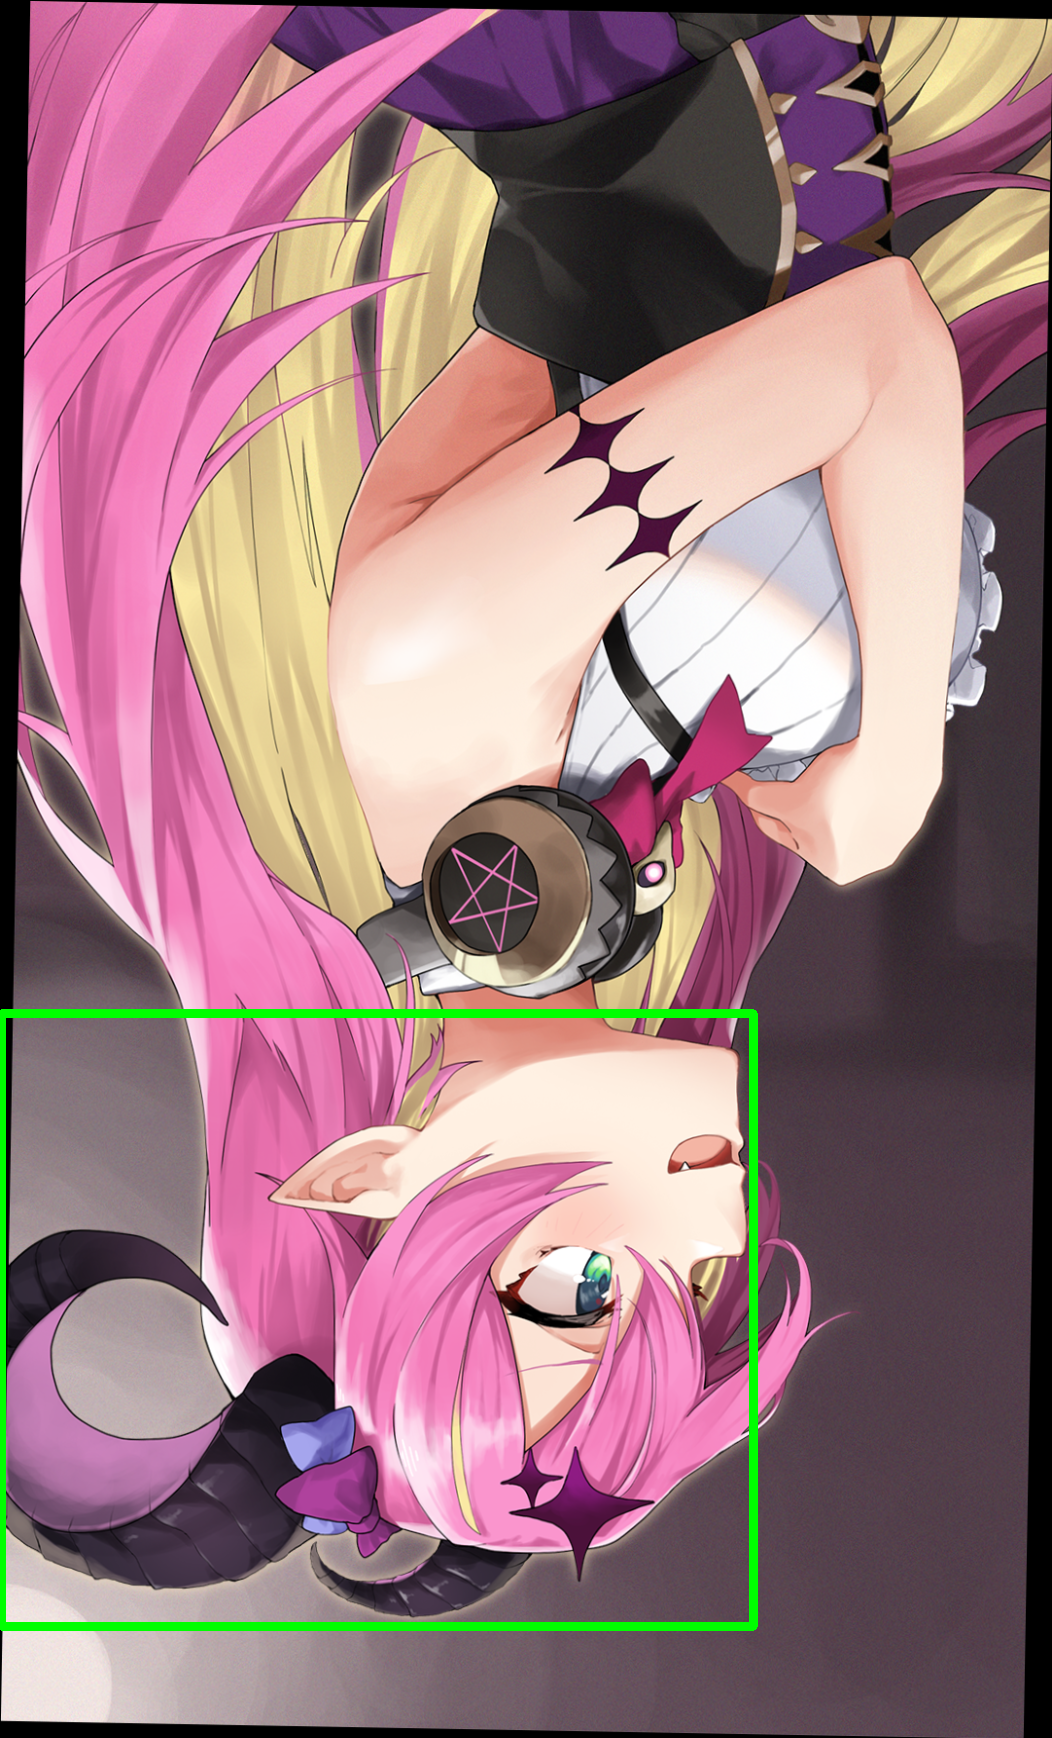
\includegraphics[width=\textwidth]{images/augmentation/Pixiv-83768702_p0-RandomRotate_179-BB.png}
        \caption{}
        \label{fig:aloe2}
    \end{subfigure}
    \hfill
    \begin{subfigure}{0.15\textwidth}
        \centering
        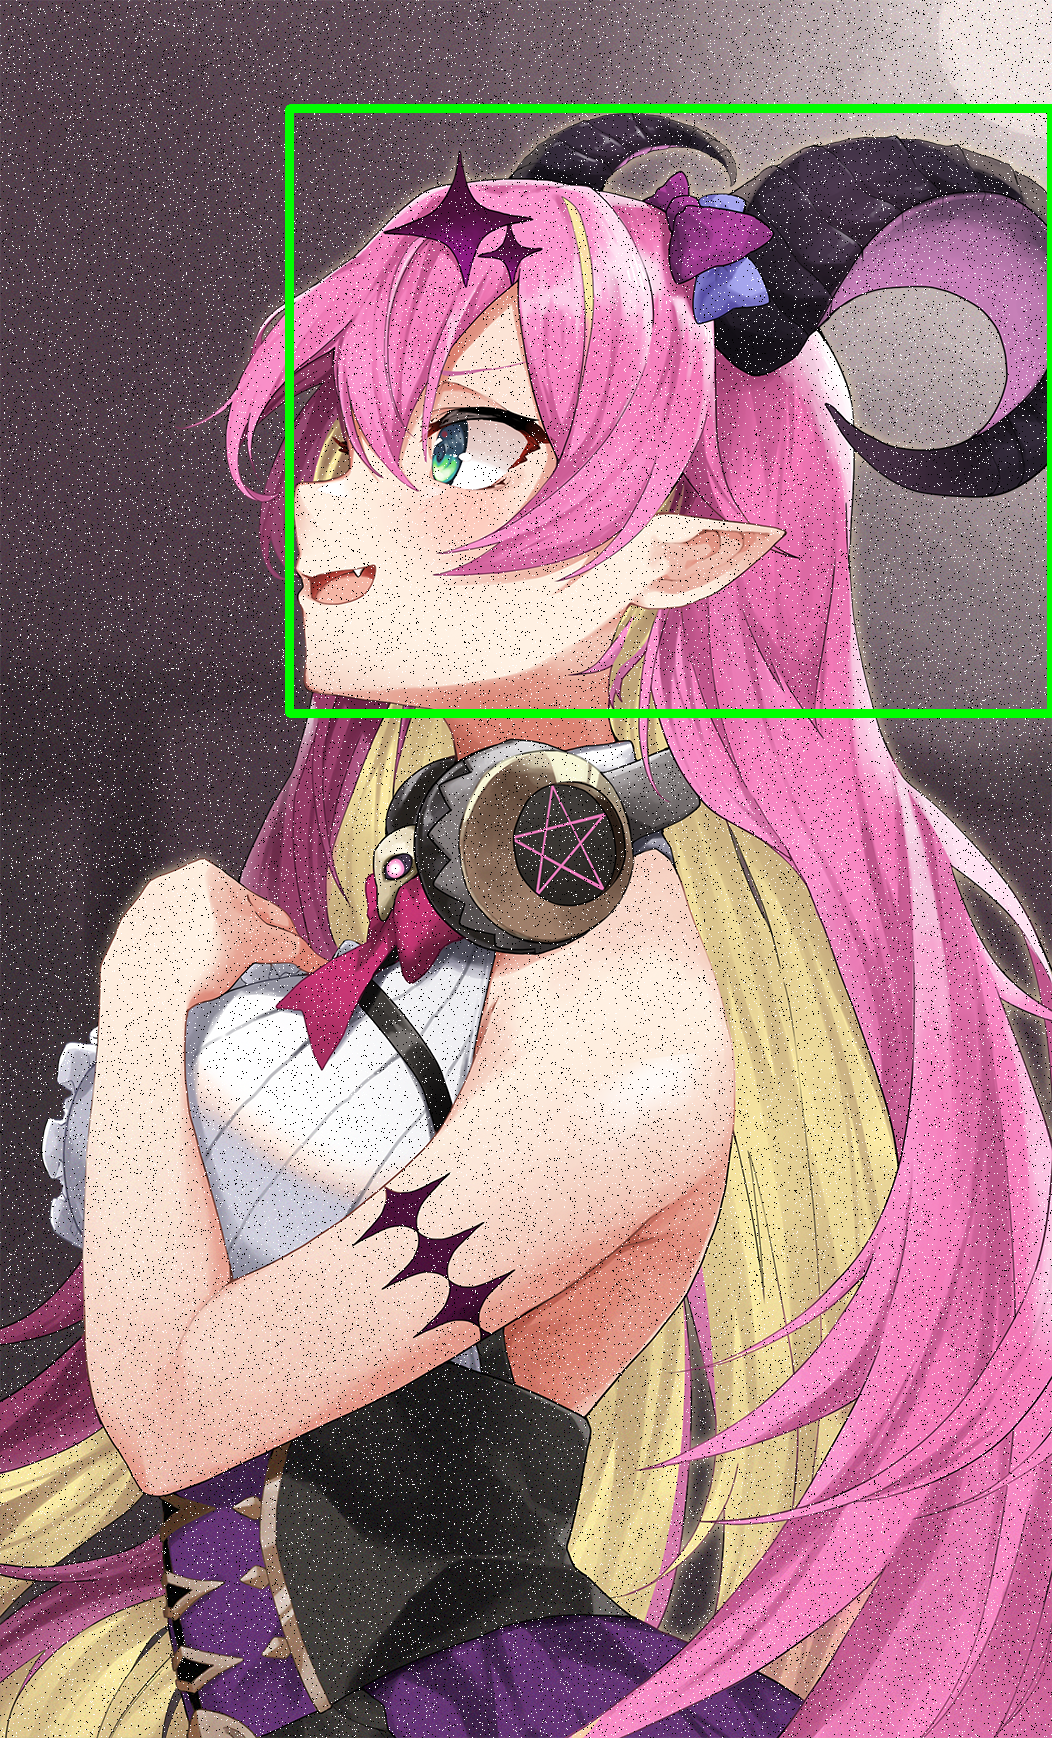
\includegraphics[width=\textwidth]{images/augmentation/Pixiv-83768702_p0-RandomSaltAndPepper_0.044-BB.png}
        \caption{}
        \label{fig:aloe3}
    \end{subfigure}
    \hfill
    \begin{subfigure}{0.15\textwidth}
        \centering
        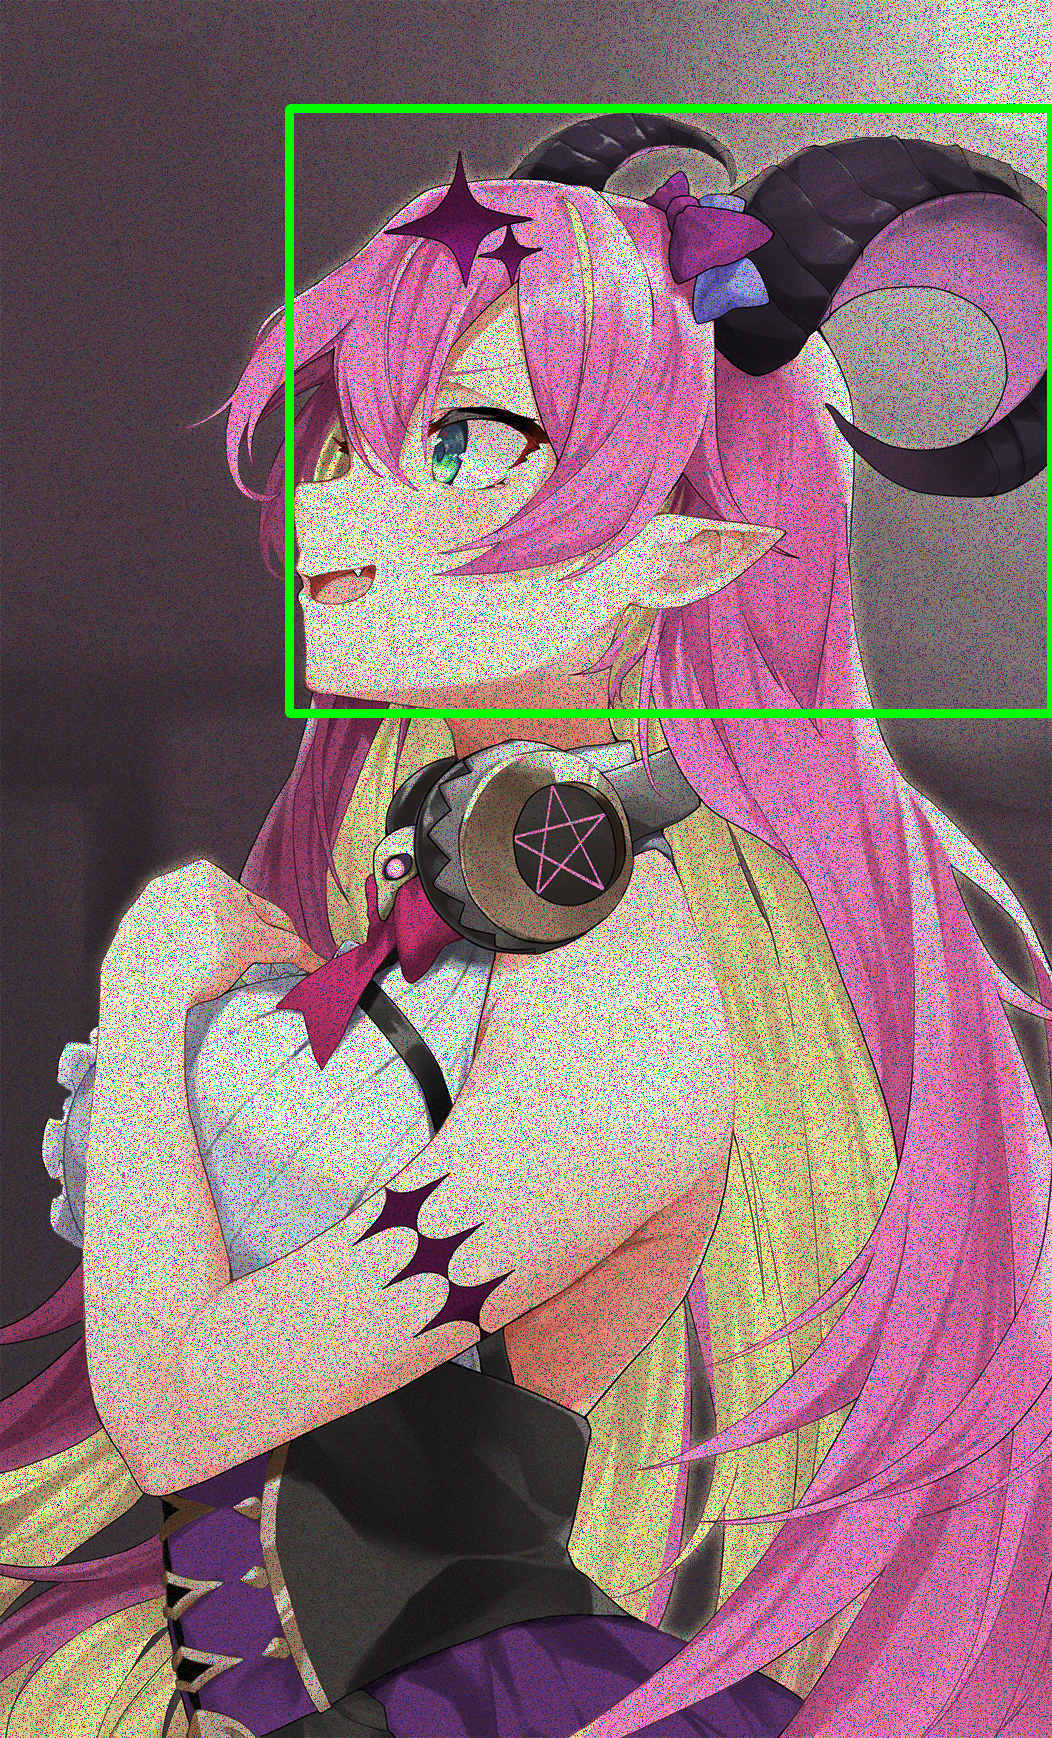
\includegraphics[width=\textwidth]{images/augmentation/Pixiv-83768702_p0-RandomValuedImpulseNoise_0.138-BB.png}
        \caption{}
        \label{fig:aloe4}
    \end{subfigure}
    \begin{subfigure}{0.15\textwidth}
        \centering
        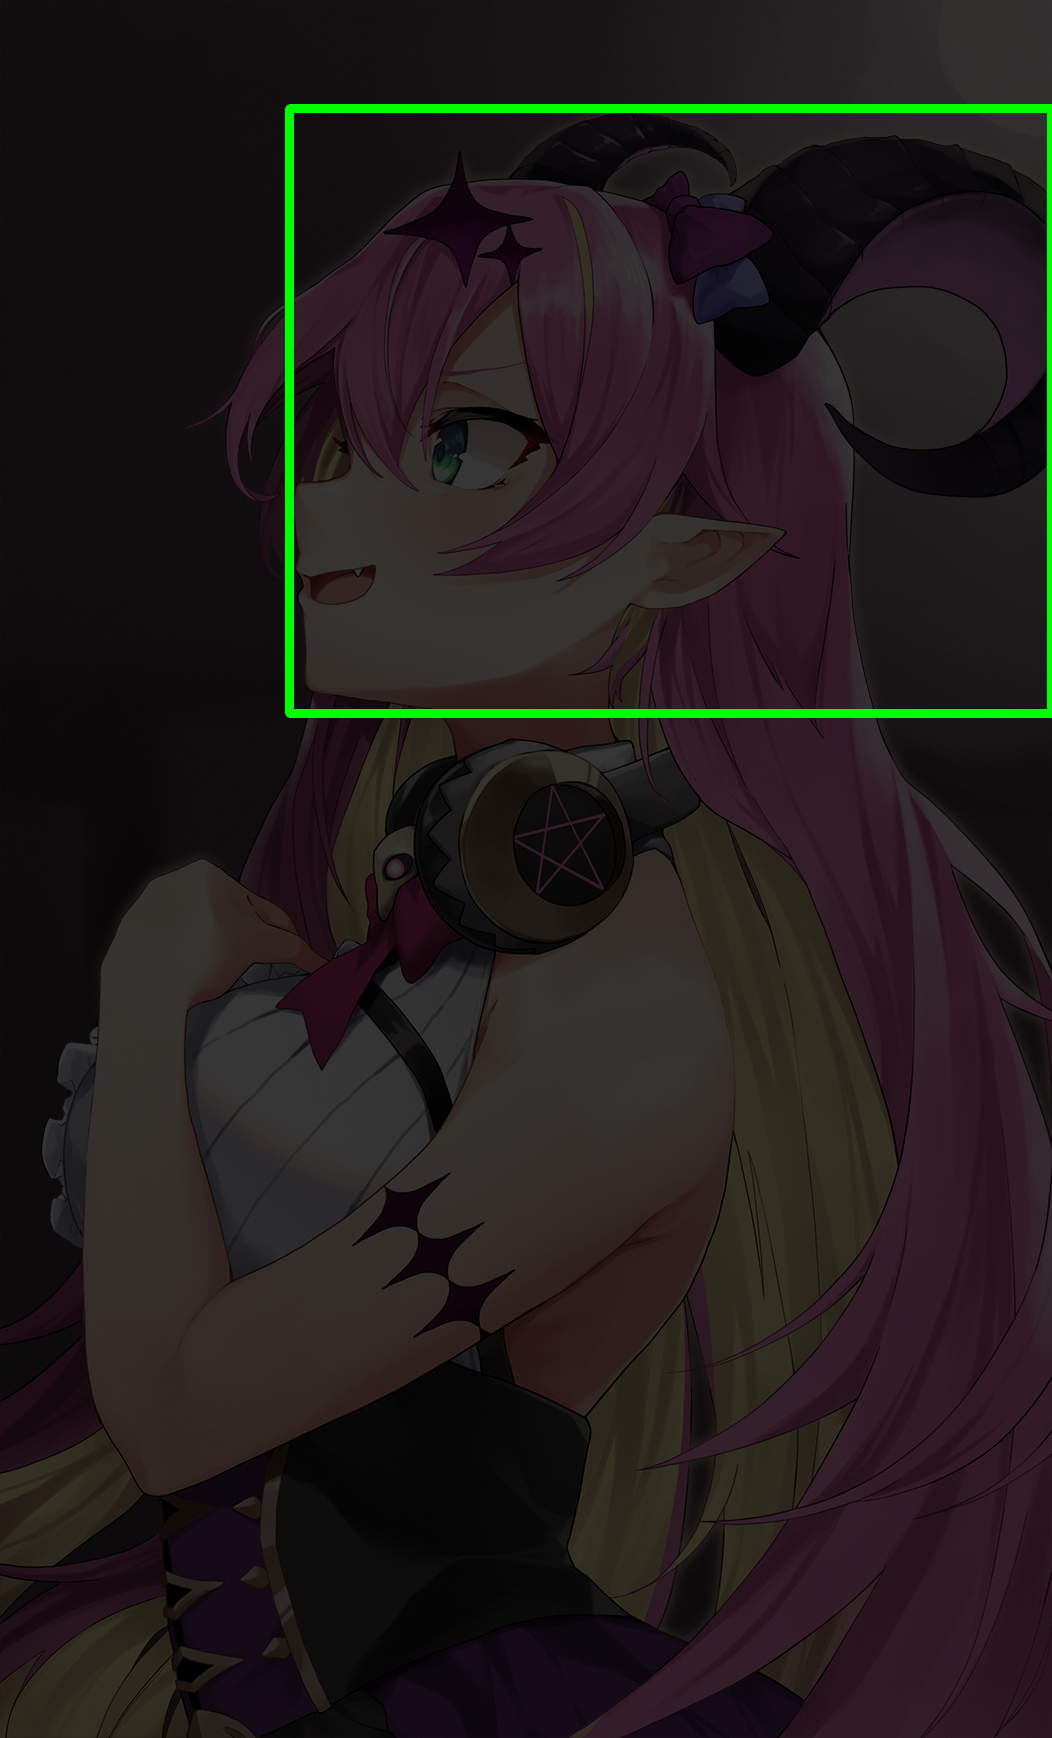
\includegraphics[width=\textwidth]{images/augmentation/Pixiv-83768702_p0-RandomBrightness_0.213-BB.png}
        \caption{}
        \label{fig:aloe5}
    \end{subfigure}
    \begin{flushleft}
        (a) Original image\cite{83768702}\\
        (b) Rotate 179 degrees\\
        (c) Random Salt and Pepper with 4.4\% \\
        (d) Random Valued Impulse Noise with 13.8\% \\
        (e) Brightness with intensity 0.213\\
    \end{flushleft}
    \caption{Data augmentation methods}
    \label{fig:manoaloe1}
\end{figure}
    \paragraph{Random-valued Impulse Noise, Salt and Pepper}
        Real-world data is seldom clean. At least it is not as clean as the data that we train our model on. 
        Noise in the data can reduce the accuracy of the model and lead to less generalization power. 
        This is the main reason why many times deep neural network models perform poorly during testing. 
        Therefore, noise are used to augment data. Not only will there be more data to use for training, 
        but the noisy data used for training the model will also make it better at generalizing real-world noisy data.
        \begin{lstlisting}[language=Python]
mask = np.random.rand(*self.image.shape[:2])
mask = np.concatenate([mask, mask, mask])
mask = mask.reshape(*mask.shape, 3)
self.image = np.where(
                self.portion*2>mask,
                np.random.randint(low=0, 
                                  high=255, 
                                  size=1, 
                                  dtype=int),
                self.image) 
        \end{lstlisting}
% =========================================================
    \paragraph{Random Brightness}
         Training the model with images with various luminosity will help it better generalize images that are not trained even on different lighting conditions\cite{RandomBrightness}. 
         The brightness and darkness depend upon one boundary value which is 1.0.
         At 1.0, the image will be in its original state.
         If the value is less than 1.0 then it will darken the image like [0.1,1.0), whereas a value greater than 1.0 makes the image brighter like (1.0, 2.0].
         At level 0 of luminosity, the image is filled with black pixels.
         \begin{lstlisting}[language=Python]
img = (self.image * self.level).astype(int)
self.image = np.clip(a=img,
                     a_min=0,
                     a_max=255)
         \end{lstlisting}
% =========================================================
    \paragraph{Image rotation}
        \label{Figure Rotation Formula}
\begin{figure}[H]
    \centering
    \includegraphics[width=0.4\textwidth]{Picture2.png}
    \label{fig:pic2}
    \begin{center}
        \begin{align*}
            N_{w} = h * \sin(\theta) + w * \cos(\theta)\\
            N_{h} = h * \cos(\theta) + w * \sin(\theta)
        \end{align*}
    \end{center}
    \caption{Rotation Formula}
\end{figure}
        \label{Figure Image Rotation}
\begin{figure}[H]
    \centering
    \begin{subfigure}{0.15\textwidth}
        \centering
        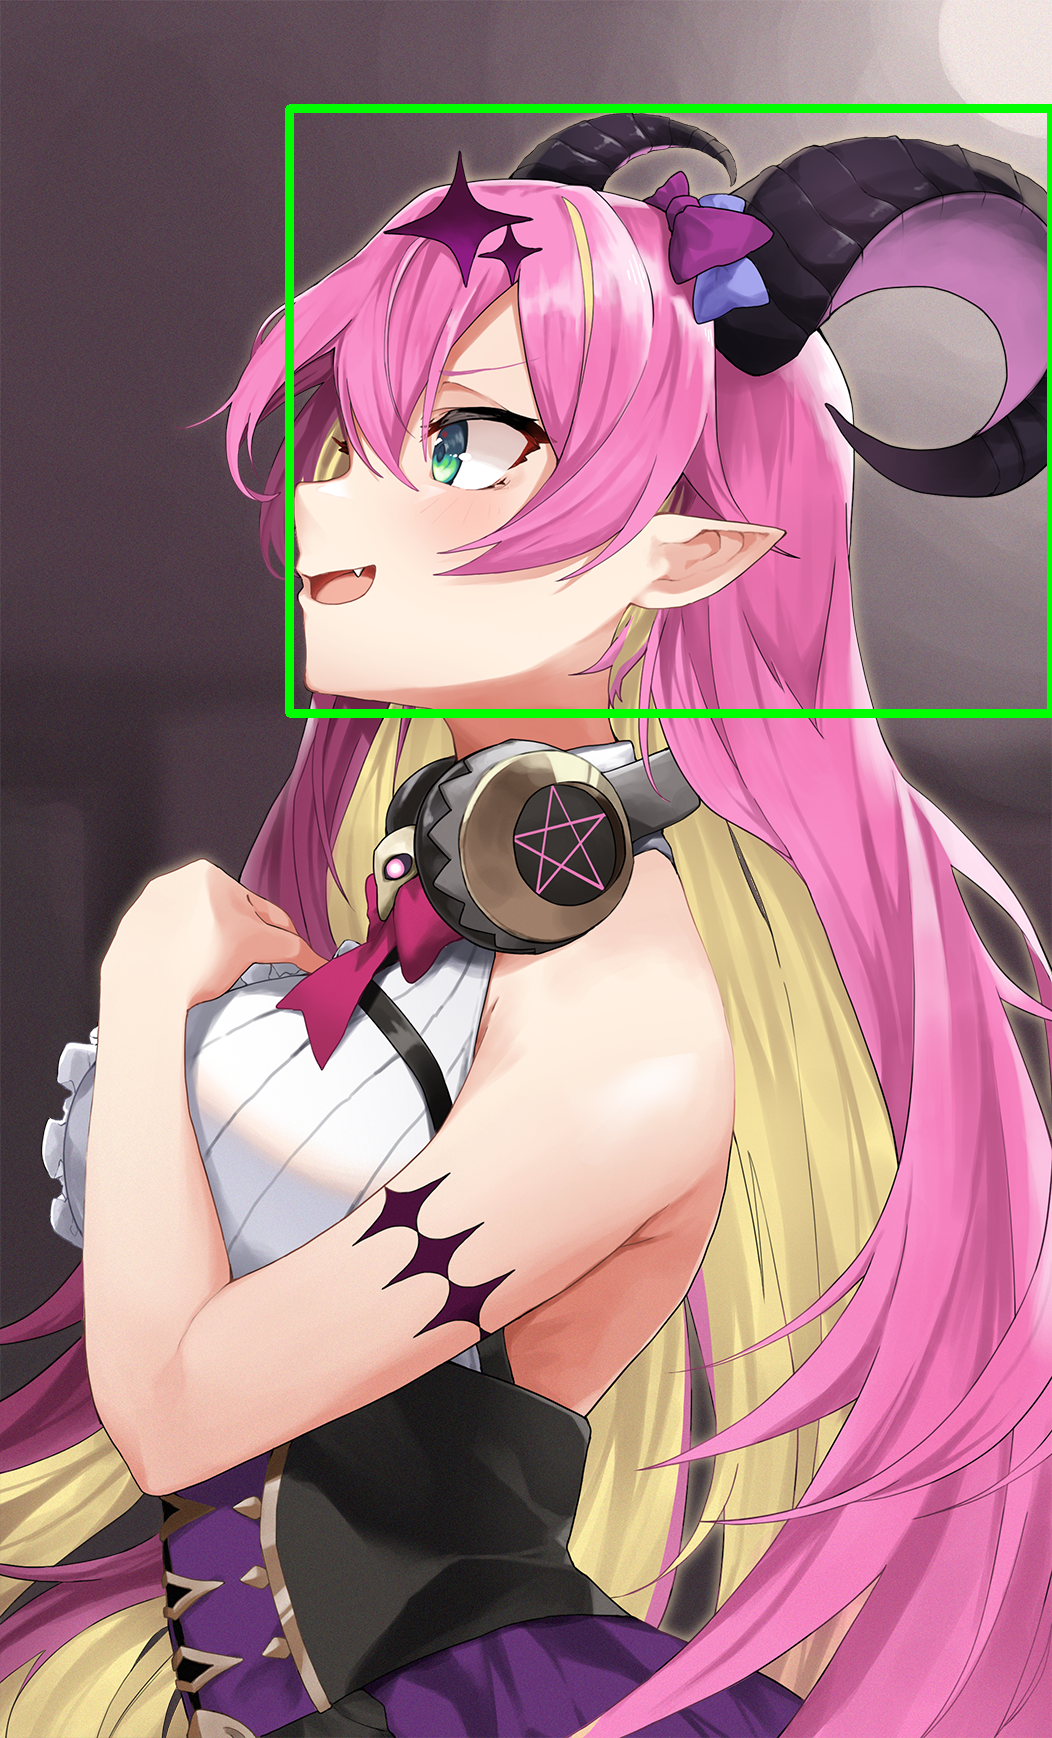
\includegraphics[width=\textwidth]{images/augmentation/Pixiv-83768702_p0-BB.png}
        % \caption{Original}
        \caption{}
        \label{fig:aloe1}
    \end{subfigure}
    \hfill
    \begin{subfigure}{0.15\textwidth}
        \centering
        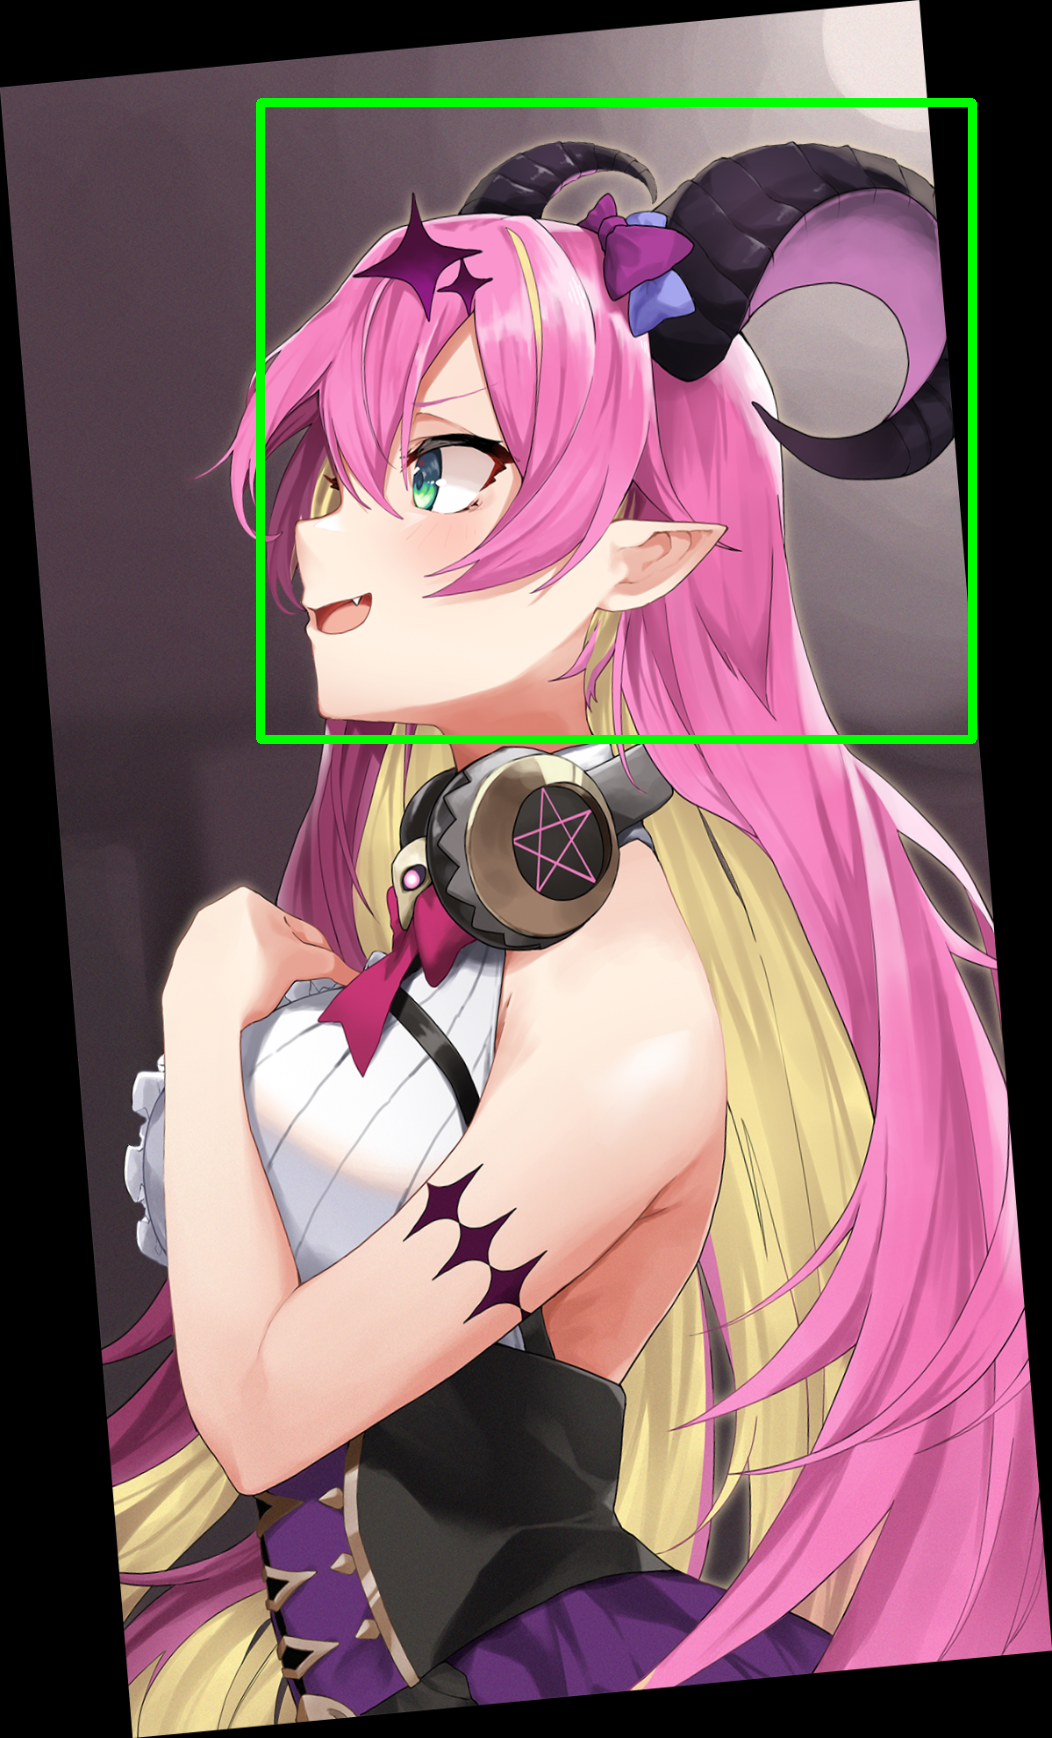
\includegraphics[width=\textwidth]{images/augmentation/Pixiv-83768702_p0-RandomRotate_5-BB.png}
        % \caption{5 degrees}
        \caption{}
        \label{fig:aloe2}
    \end{subfigure}
    \hfill
    \begin{subfigure}{0.15\textwidth}
        \centering
        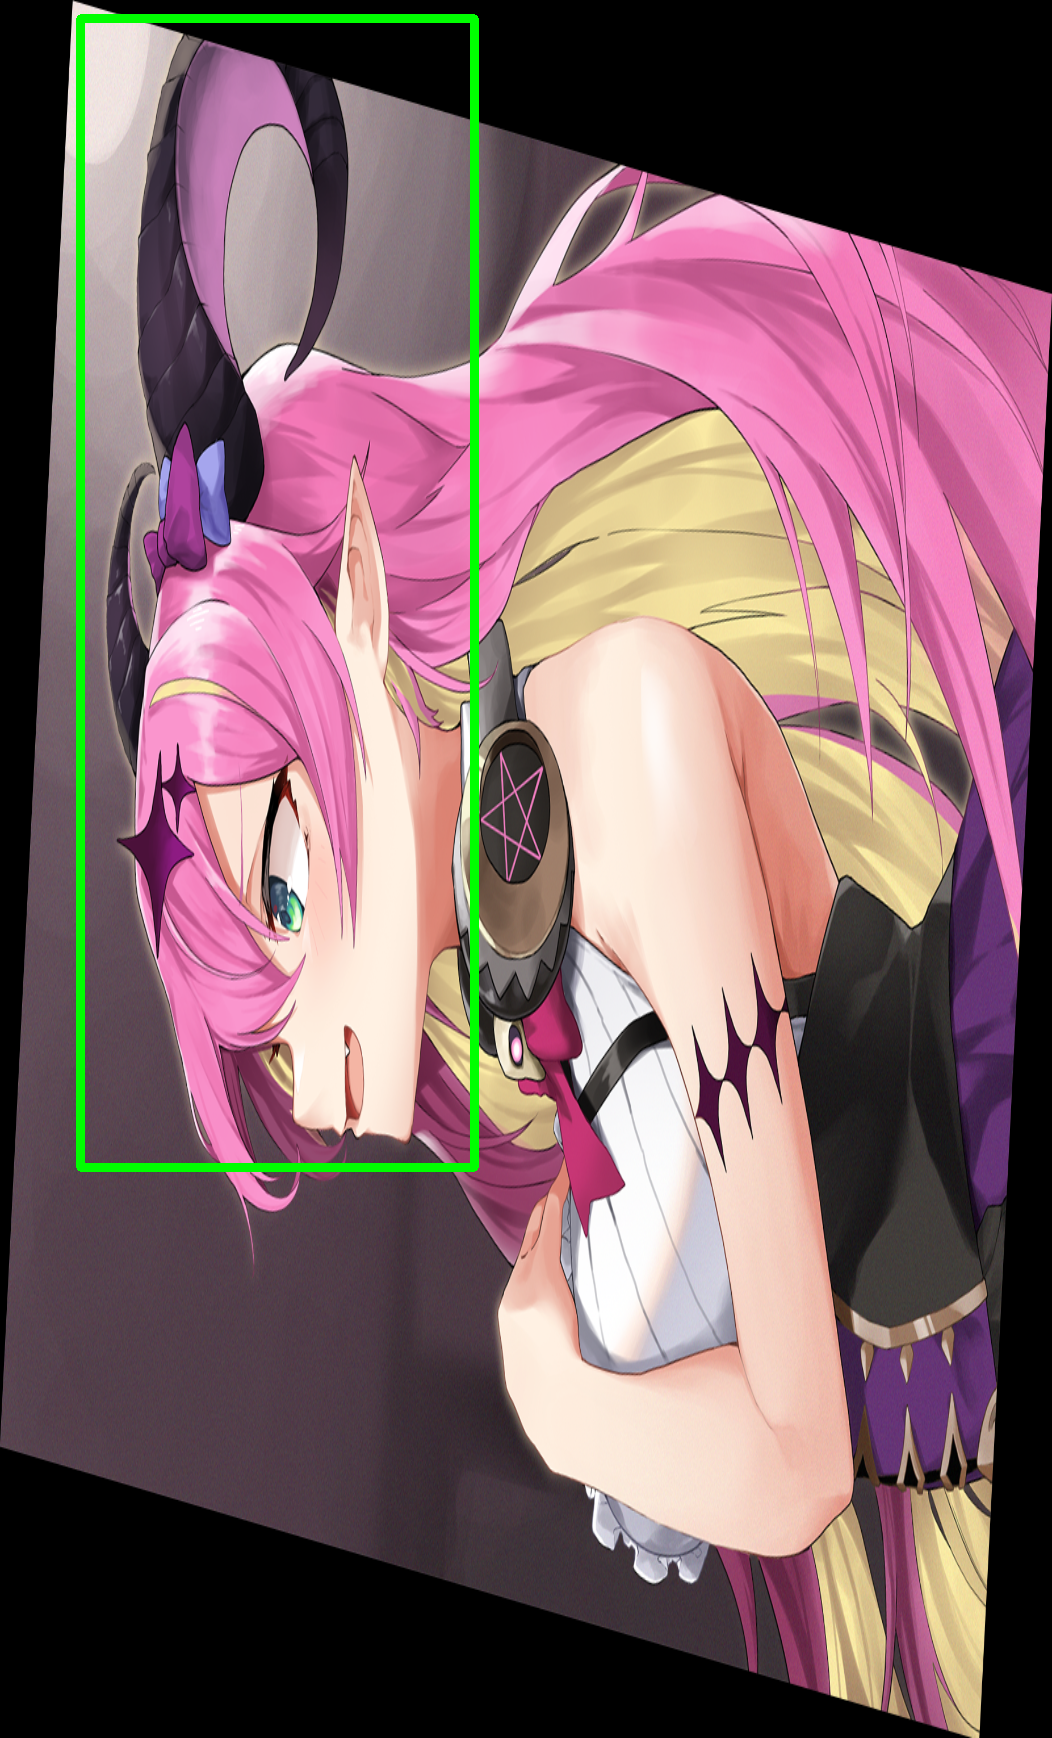
\includegraphics[width=\textwidth]{images/augmentation/Pixiv-83768702_p0-RandomRotate_83-BB.png}
        % \caption{83 degrees}
        \caption{}
        \label{fig:aloe3}
    \end{subfigure}
    \hfill
    \begin{subfigure}{0.15\textwidth}
        \centering
        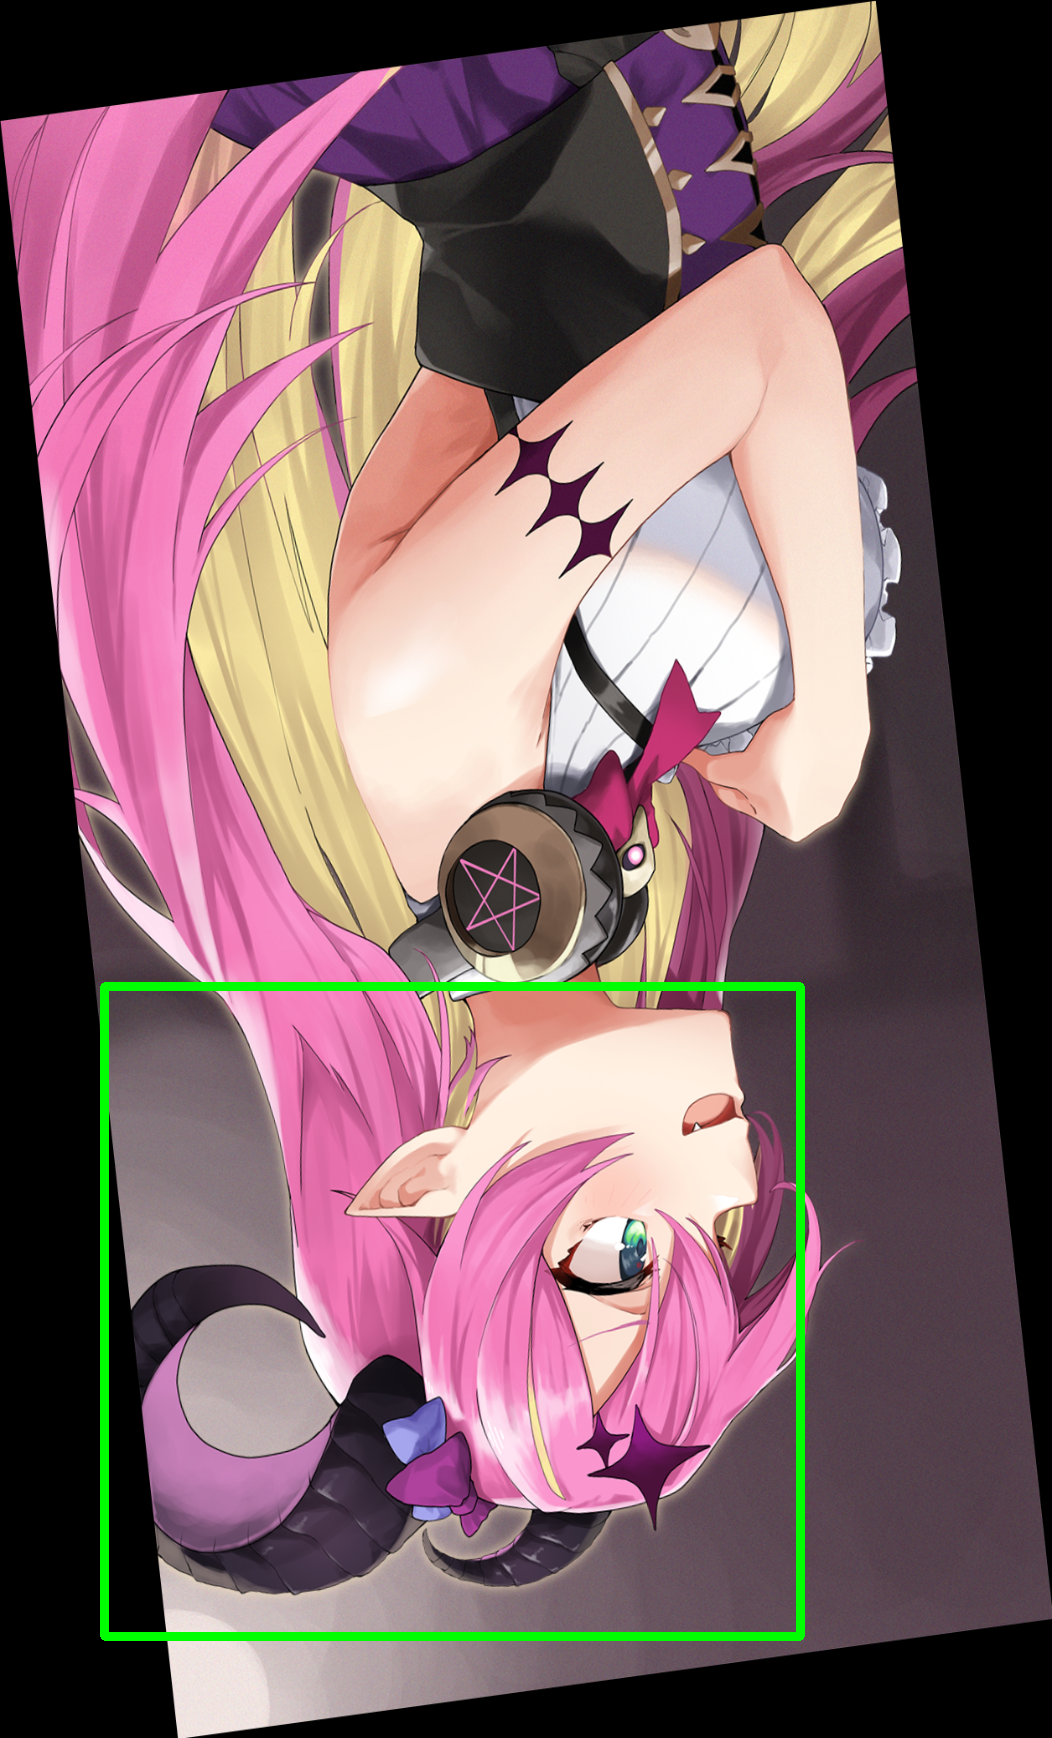
\includegraphics[width=\textwidth]{images/augmentation/Pixiv-83768702_p0-RandomRotate_187-BB.png}
        % \caption{187 degrees}
        \caption{}
        \label{fig:aloe4}
    \end{subfigure}
    \begin{subfigure}{0.15\textwidth}
        \centering
        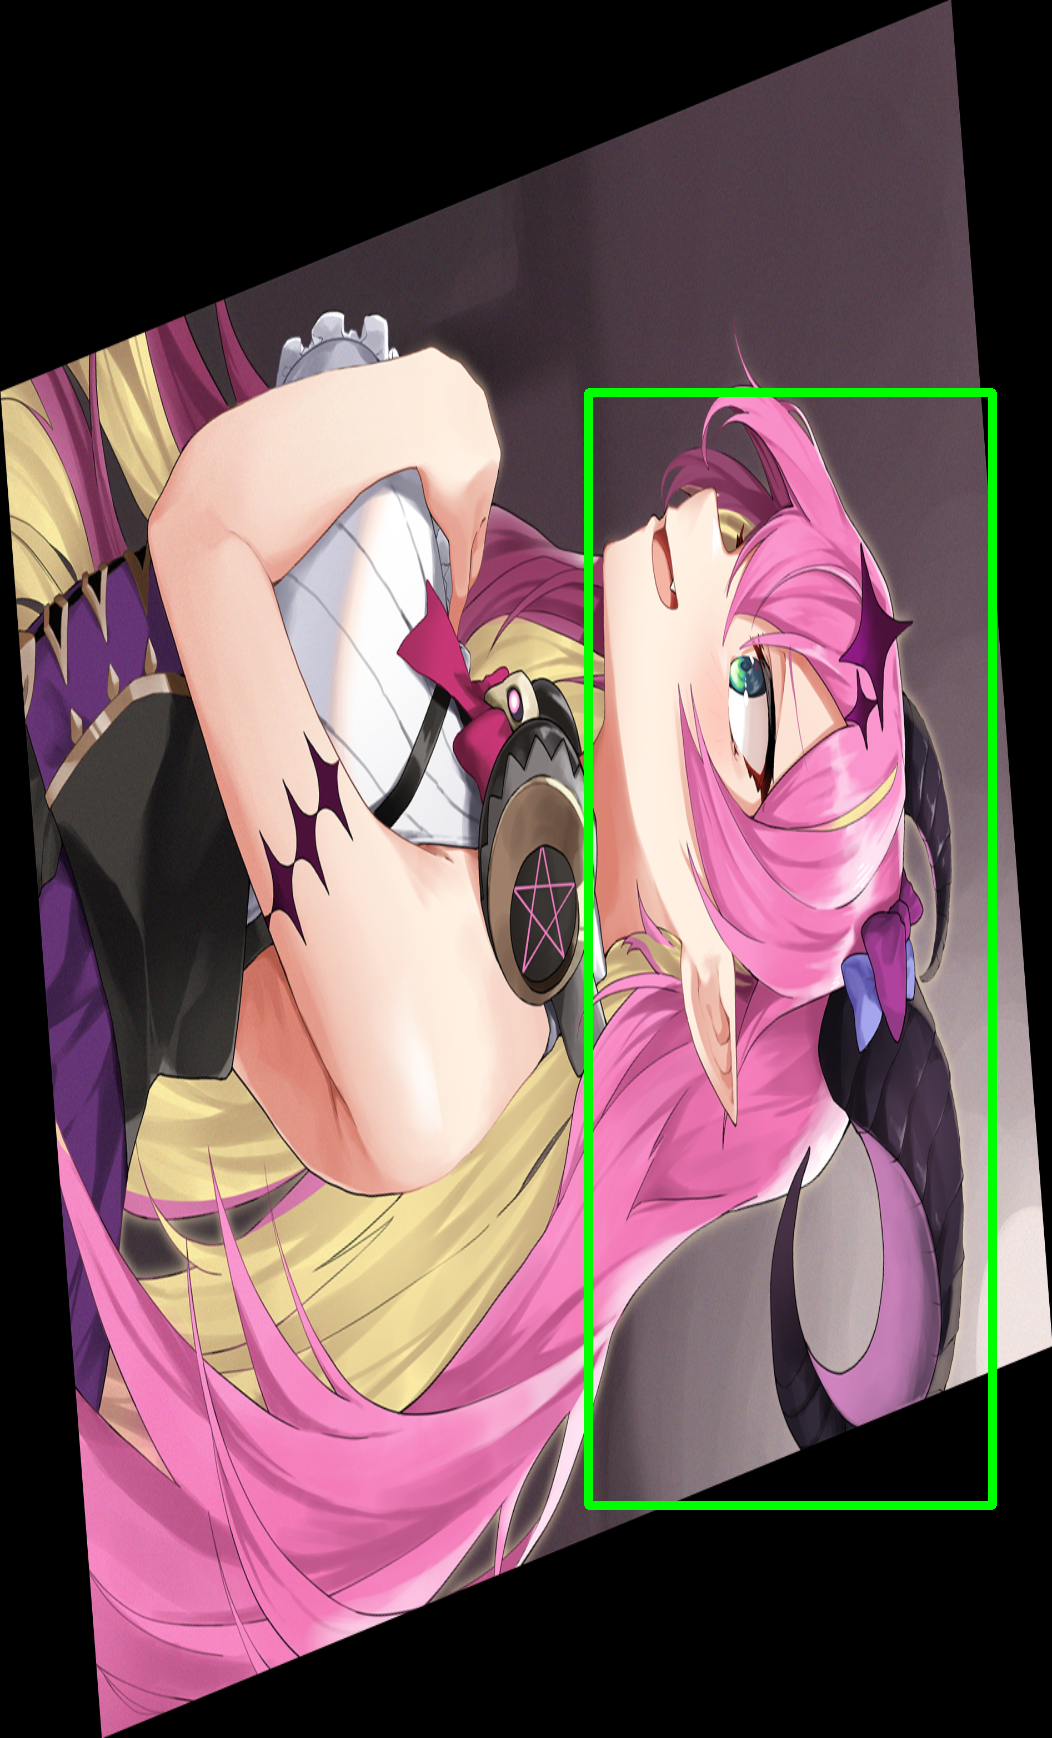
\includegraphics[width=\textwidth]{images/augmentation/Pixiv-83768702_p0-RandomRotate_280-BB.png}
        % \caption{280 degrees}
        \caption{}
        \label{fig:aloe5}
    \end{subfigure}
    \begin{flushleft}
        (a) Original image\cite{83768702}\\
        (b) Rotate with 5 degrees\\
        (c) Rotate with 83 degrees\\
        (d) Rotate with 187 degrees\\
        (e) Rotate with 280 degrees\\
    \end{flushleft}
    \caption{Image Rotation}
    \label{fig:manoaloe1}
\end{figure}
        Because it alters the angles at which objects appear in the dataset during training, Random Rotate is a particularly helpful augmentation. 
        Perhaps images were only taken with an item horizontally throughout the image gathering phase, but the object could have been skewed in any direction during manufacturing. 
        However, this method is by far the most sophisticated. 
        The items in an image are also relocated when it is rotated.
        However fortunately, we discovered a tutorial by Ayoosh Kathuria that can assist us in solving this issue with just some modification\cite{Rotation}.          
            \subsubsection{Adding Backgorund}
    Background images are those that do not have an object that needs to be classified to reduce False Positives (FP).
    Small chunks of background images are added to the training, validation, and testing datasets in addition to labeled images.
    As the background image fraction approaches 1.0, the training process will suffer.
    Background images should have a maximum proportion of 10 percent, as recommended by the author of YOLO5.
    In this project, background should be scenery images\cite{addingbackgroundimages}. 
    \begin{figure}[H]
    \centering
    \begin{subfigure}{0.241\textwidth}
        
\includegraphics[width=1\textwidth]{images/background/Pixiv-101510980_p0.png}
    \end{subfigure}
    \hfill
    \begin{subfigure}{0.241\textwidth}
        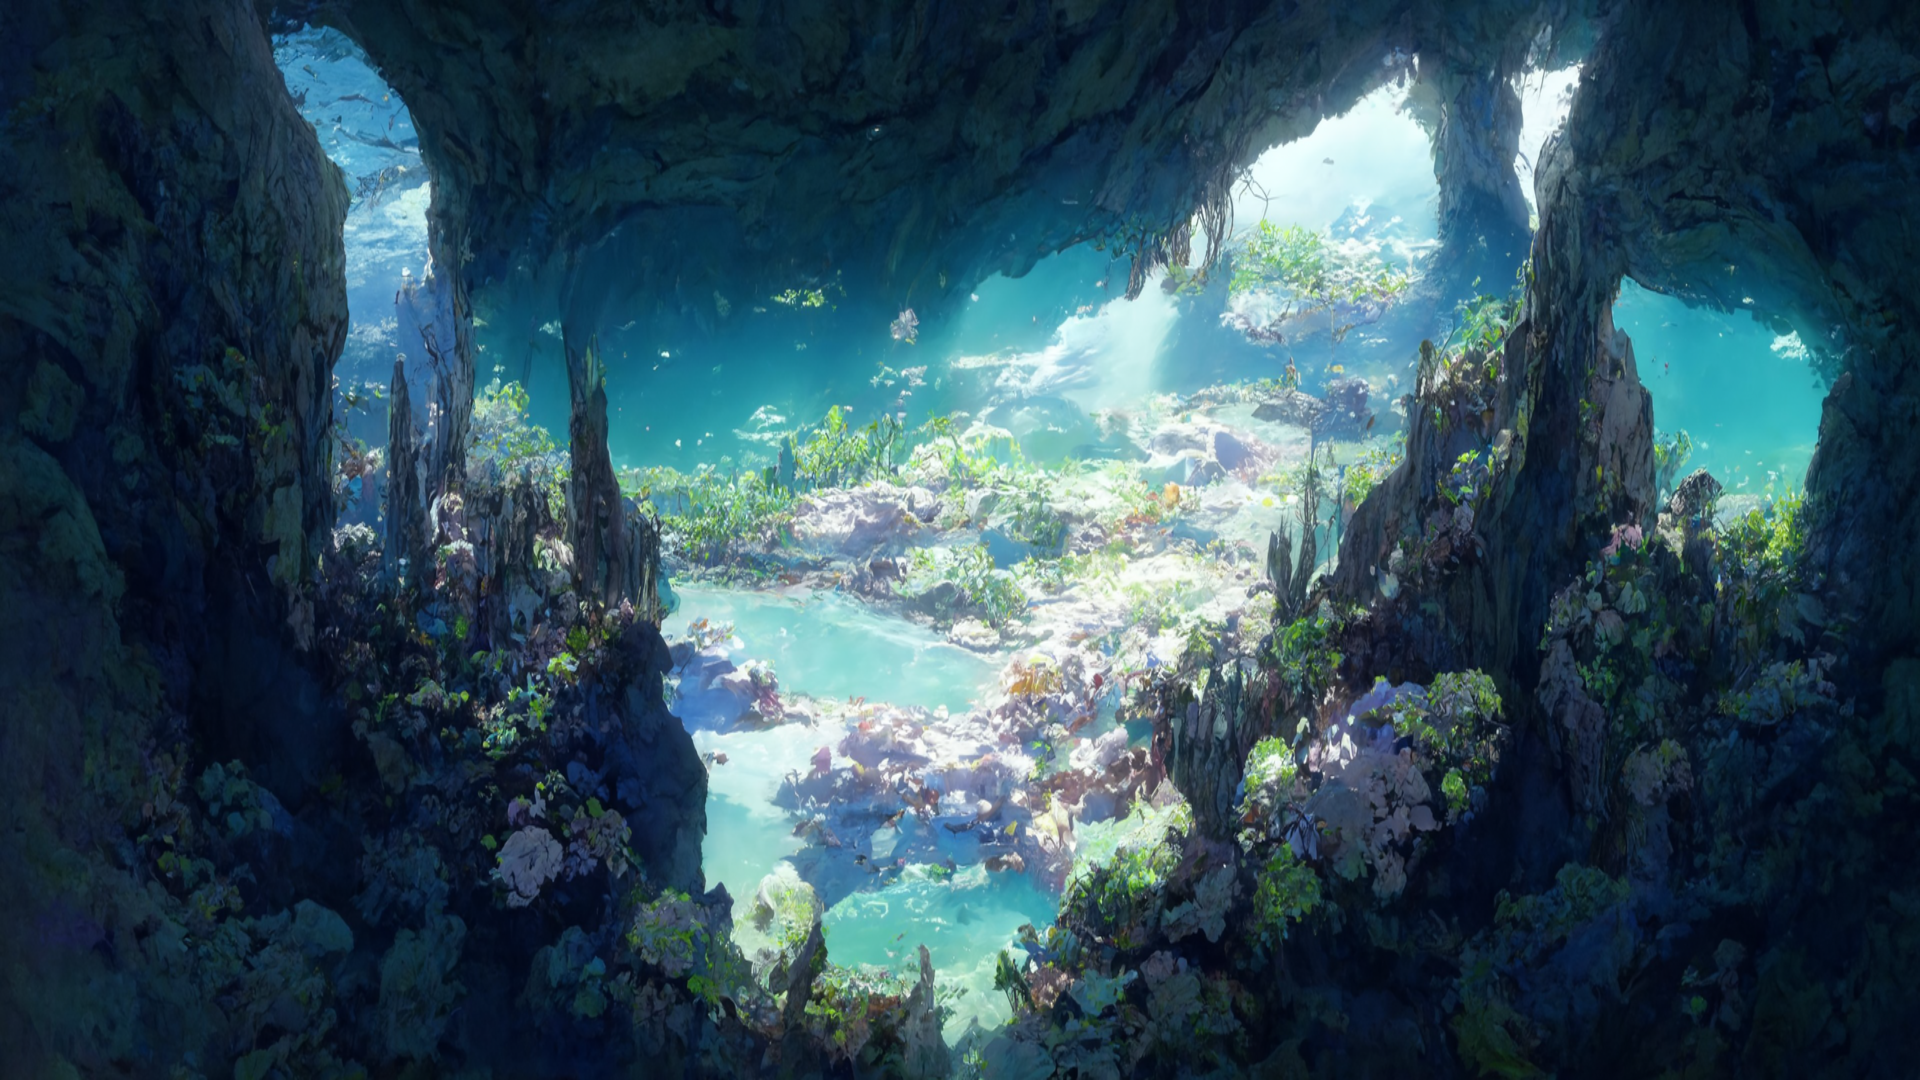
\includegraphics[width=1\textwidth]{images/background/Pixiv-100810147_p2.png}
    \end{subfigure}
    \hfill
    \begin{subfigure}{0.241\textwidth}
        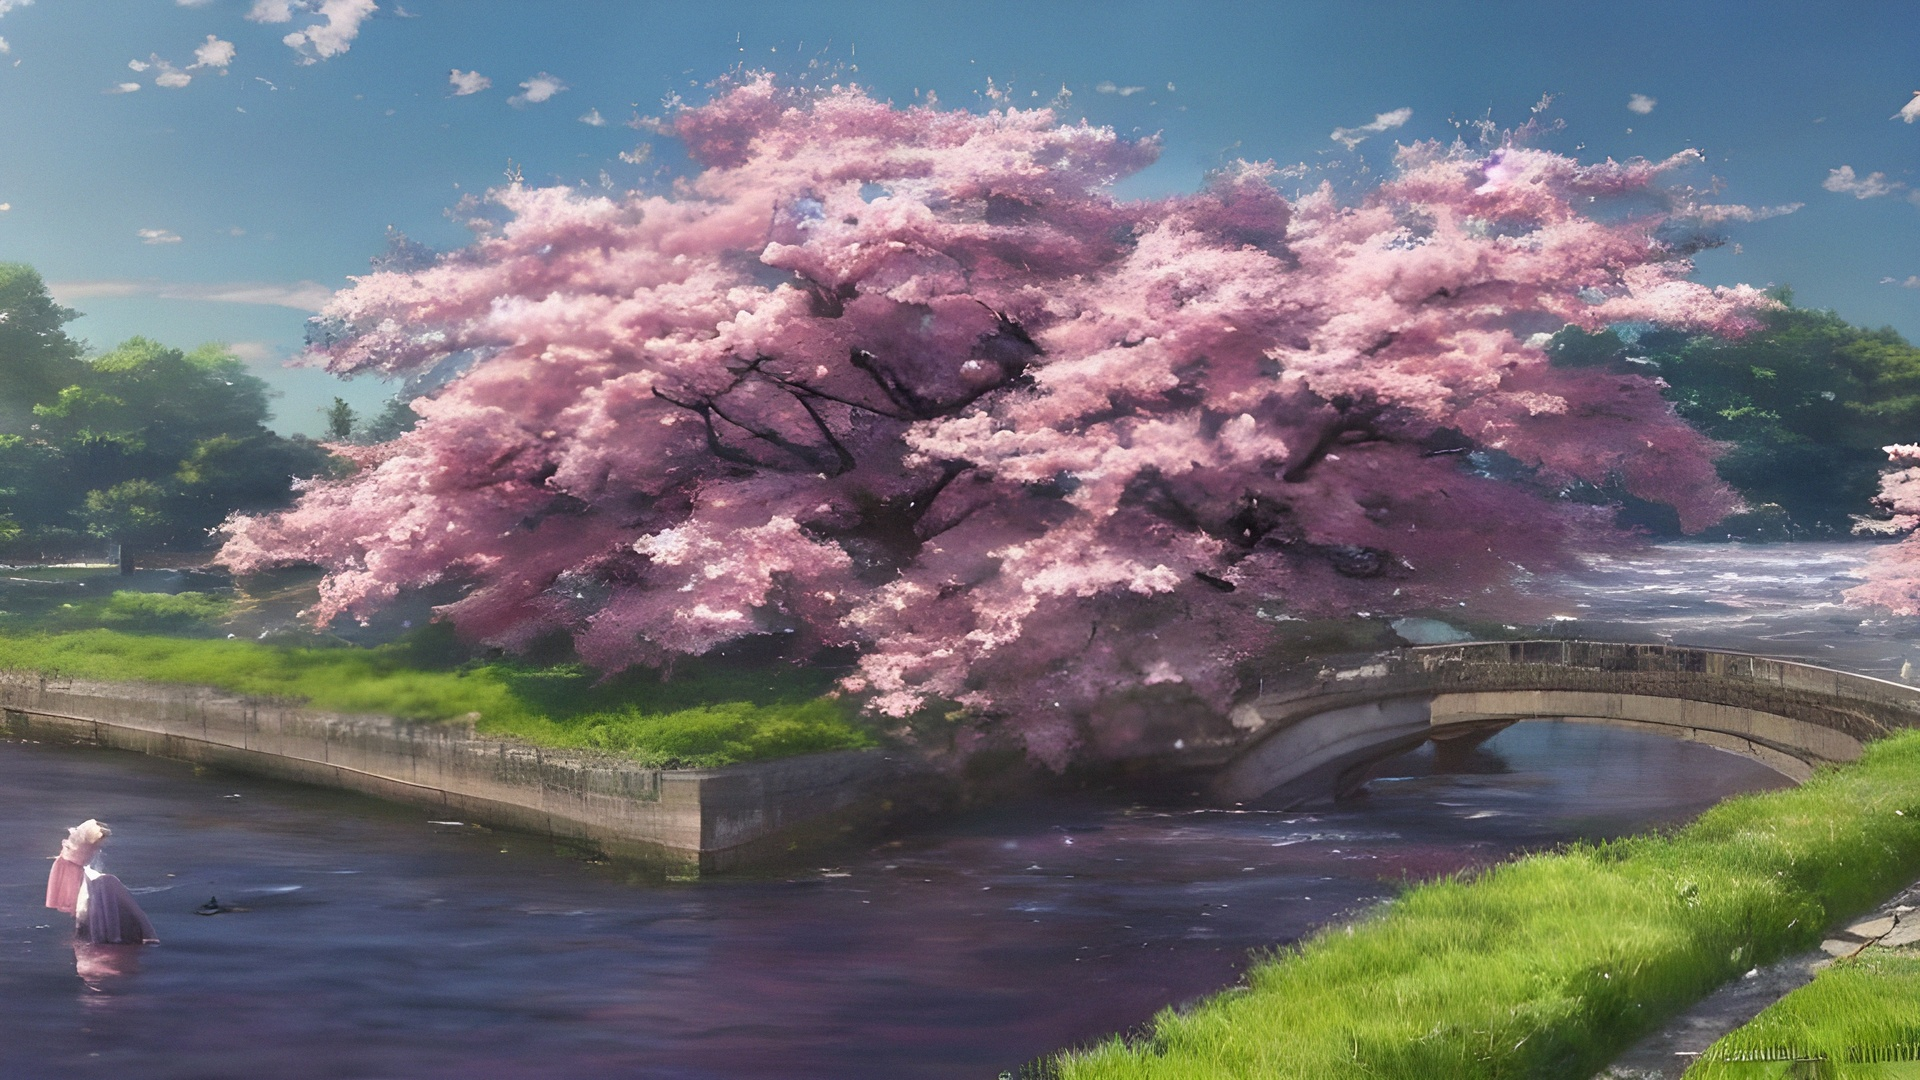
\includegraphics[width=1\textwidth]{images/background/Pixiv-101735564_p0.jpg}
    \end{subfigure}
    \hfill
    \begin{subfigure}{0.241\textwidth}
        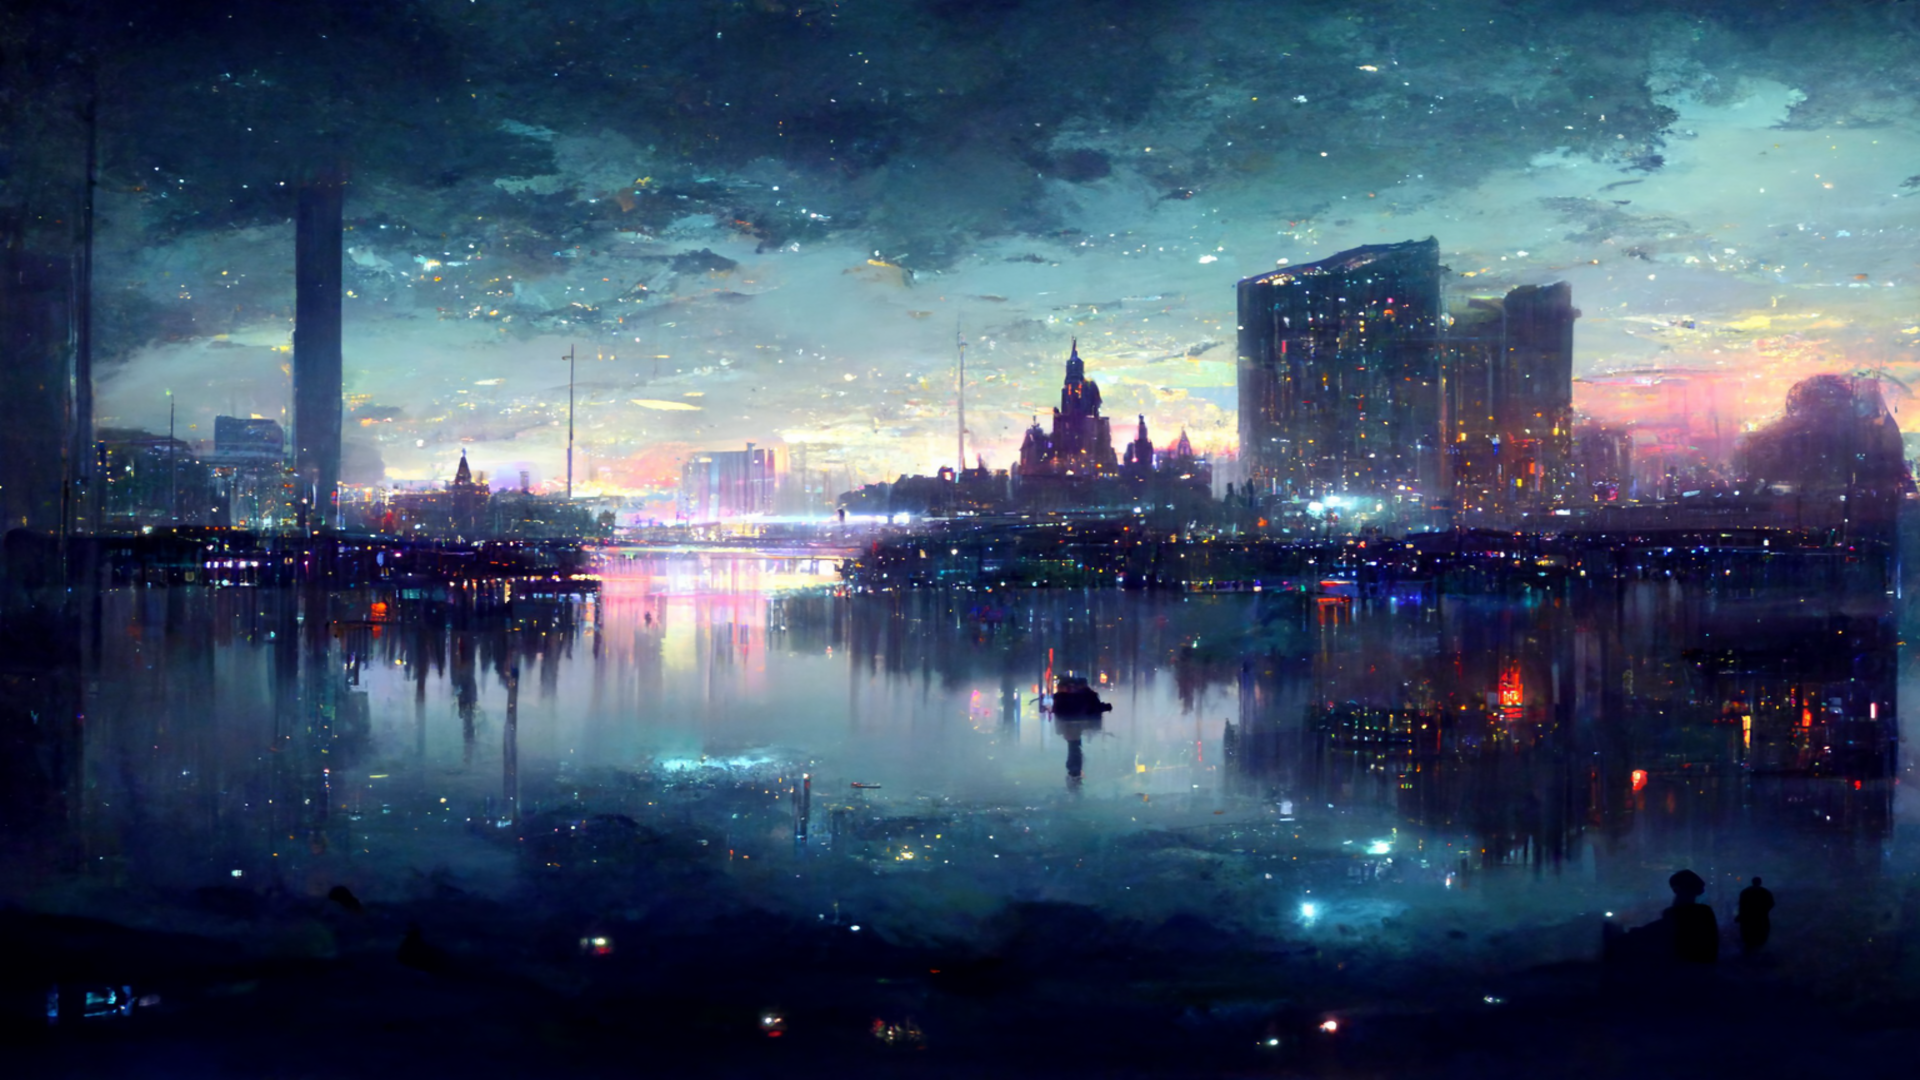
\includegraphics[width=1\textwidth]{images/background/Pixiv-101752160_p1.png}
    \end{subfigure}
    \caption{Background images\cite{101510980}\cite{100810147}\cite{101735564}\cite{101752160}}
\end{figure}
% ================================================================================================= 
        \subsection{Evolving Hyperparameter}
        Hyperparameter is the type of parameter whose values govern the entire deep learning model's learning process. 
        Furthermore, it determines the values of model parameters that a learning algorithm ends up learning, despite not being a part of the deep learning model.

        Hyperparameter evolution is a method of hyperparameter optimization that employs a Genetic Algorithm (GA) for optimization.
        In machine learning, hyperparameters control numerous elements of training, and finding optimal values for them may be complex. 
        Traditional approaches, such as grid searches, can soon become intractable owing to the large dimensionality of the search space, unknown relationships across dimensions, and the costly aspect of evaluating fitness at each point, making GA a viable choice for hyperparameter searches\cite{EvolvingHyperparameter}.
% ================================================================================================= 
        \subsection{Traning and Inference}
            Through training, data is fed into the model to produce a better-trained model. The new weight is then used to infer unlabeled images. That made the labeling procedure faster and less tedious.
%           ================================================================================================= 
        \subsection{Manually Check Label}
            After all of the images have been processed, the 
            identity of each face within each image will be manually checked and adjusted using \textbf{labelImg}\cite{labelimg} to set a better standard for the 
            face detection model. These images along with the bounding box and identity 
            data will then be used for our face identification model. The restrictions for the bounding box span from the top of the head to the chin and ear-to-ear; if they have certain unique accessories, those are also included.
% ================================================================================================= 
        \subsection{Label Format}
            YOLOv5 Pytorch has a highly unique label format. (\autoref{fig:yolov5format}). 
            Therefore, this format must be converted to another standard format, like Pattern Analysis Statistical Modeling and Computational Learning Visual Object Classes (Pascal VOC)\cite{pascalvoc} or Common Objects in Context (COCO)\cite{coco} (\autoref{fig:otherformats}), when interacting with other processes, like rotation in augmentation.
            For this reason, a different sub-program called \textbf{Bounding Box Converter}\cite{boundingboxconverter} was developed using the formulas shown in \autoref{fig:conversionformula}. Here is the snippet of how it was implemented: \autoref{fig:thefillerarc}.